\section{Interactive System}


\begin{figure}[ht]
\centering
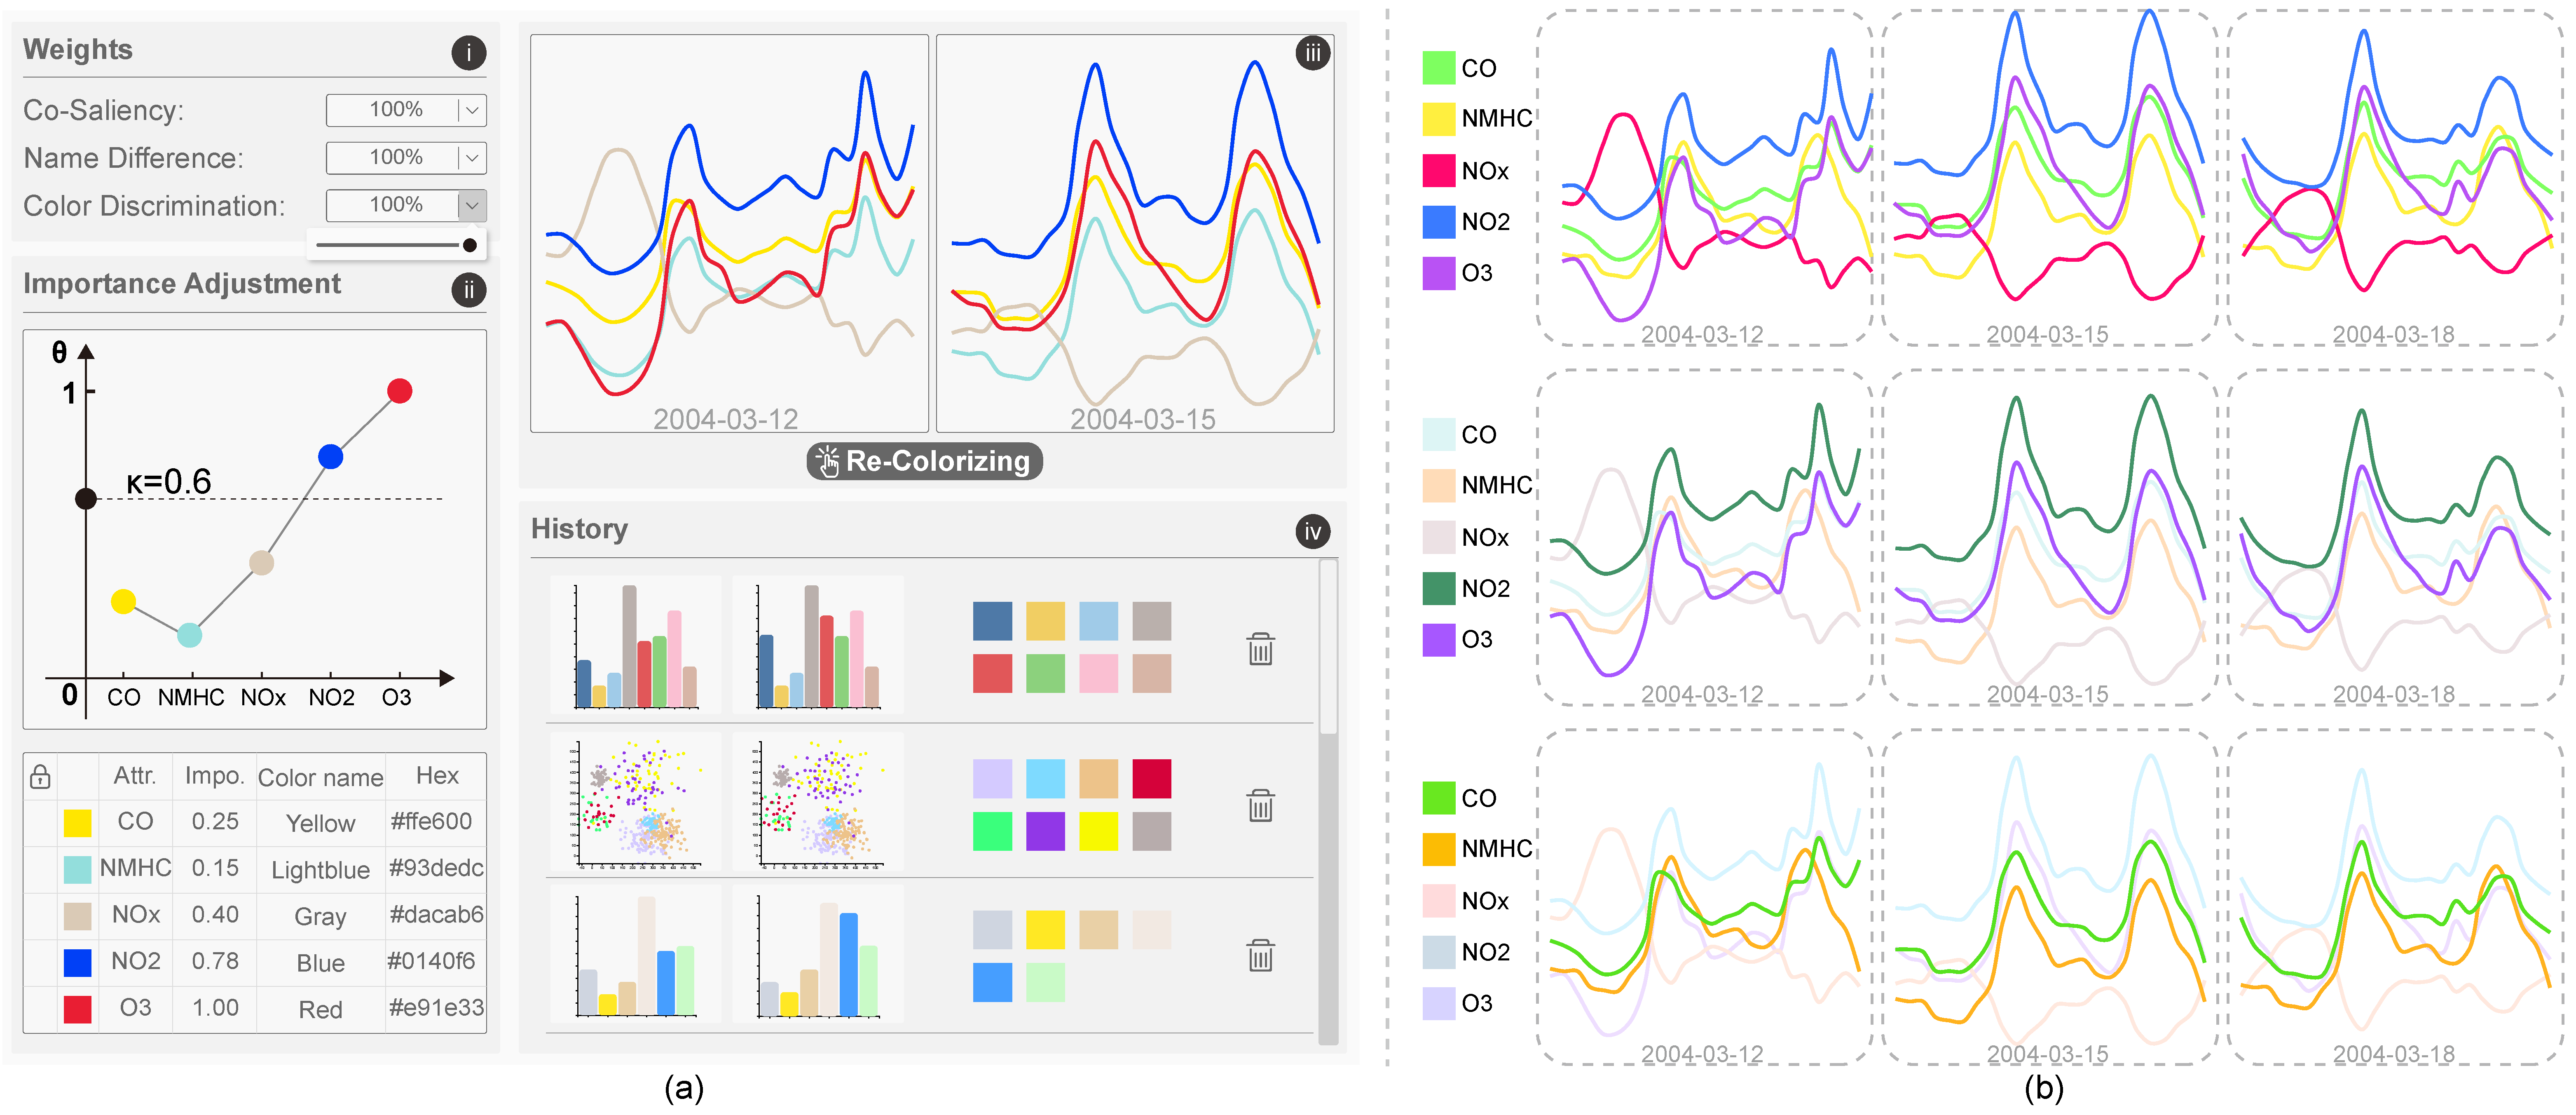
\includegraphics[width=1.0\columnwidth]{figures/interface.pdf}
\caption{Our interactive colorization system and a case study. (a) Screenshot of the interactive system consisted of four panels: (i) control panel; (ii) importance adjustment panel; (iii) visualization panel; and (iv) history panel. (b) Using this system to explore the changes of gases in an air quality data set~\cite{DEVITO2008750}: (top) The automatic generated palette creates salient colors for  lines; (middle, bottom) the palettes highlighting two lines with small changes generated by our methods without and with colour name constraint, respectively.}
\vspace*{-3mm}
\label{fig:ui-case}
\end{figure}

%\subsection{Interactive System}
\label{sec:interaction}
To help users interactively design colors for comparing multi-class scatterplots, we developed a web-based multi-view visualization tool \footnote{\small \url{https://c3-palette.github.io/}}
(see the screenshot in Fig.~\ref{fig:ui-case}(a)).
It consists of four coordinated views: (i) a control panel, (ii) an importance adjustment panel for adjusting $\kappa$ and  importance of each class, (iii) the juxtaposed visualizations, and (iv) a history view. 

After uploading multiple labeled datasets, the system automatically finds an optimal color mapping scheme to colorize the input data, while each class is encoded as a dot on the x-axis of the importance adjustment view indicating the change degree. If users like the color mapping scheme, they can save it to the history view. By default, our system finds a color mapping scheme to highlight the classes with large changes and renders the classes in ascending order of the corresponding change degrees. 
To facilitate a coherent exploration, we provide a color name constraint for  palette generation, where the consistency of color names will be preserved in the produced palettes.
If users like the color mapping scheme, they can save it to the history view.









\vspace{1.5mm}
\noindent\textbf{Color Name Constraints}.
Adjusting class importance and $\kappa$  allows to highlight some classes of interest with newly generated color palettes. However, this might not be intuitive for users, since the colors might be completely changed in the new palette. To address this issue,
one straightforward way is to  assign large  opacities  to classes of interest and small values to deemphasized classes, respectively. However, this method might not be able to pop out such classes, since their assigned colors are often have low contrast with the background (e.g., the yellow class in the top of Fig.~\ref{fig:ui-case}(b)).

To maintain consistent color schemes and highlight classes of interest, we introduce a color name constraint~\cite{heer2012color} for palette generation. Specifically, the name difference between the new color and the one in the previous palette should be smaller than a threshold during the search for new palettes.
In doing so, such selected classes can be easily identified from the new colorization results (see an example in the bottom of Fig.~\ref{fig:ui-case}(b)).




\subsection{Case Study}
\label{sec:caseStudy}


%\begin{figure}[!t]
%\centering
%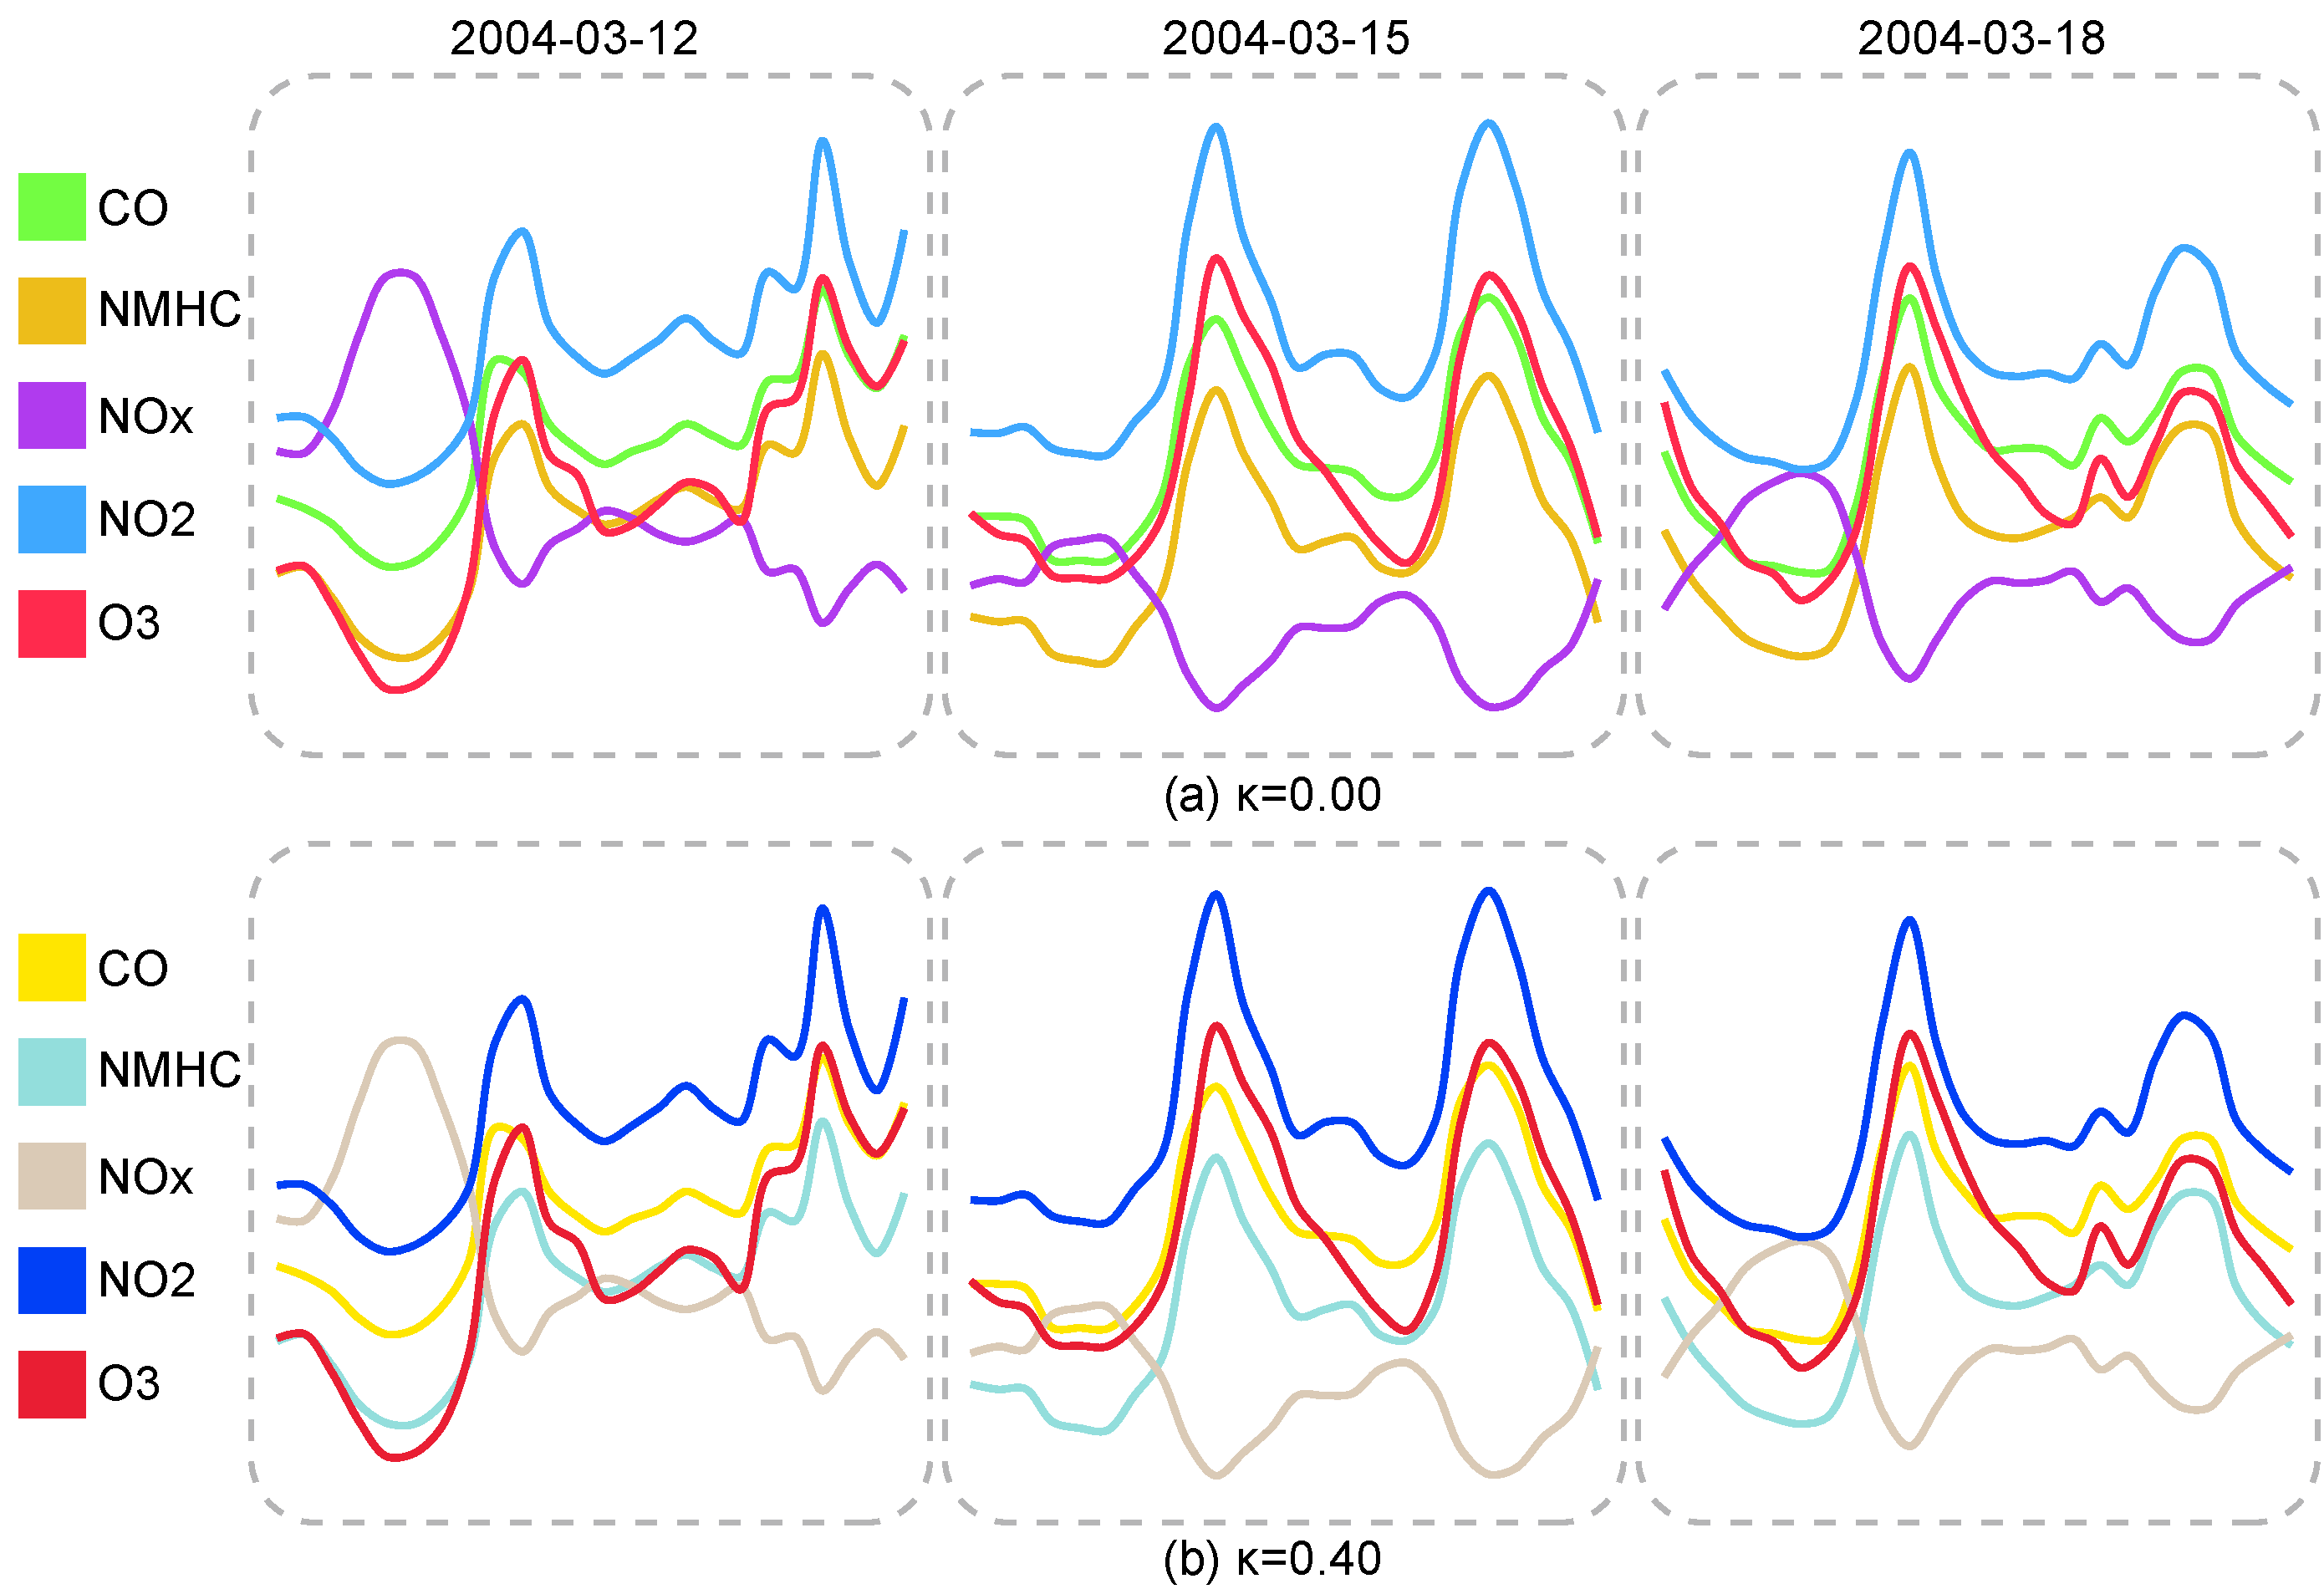
\includegraphics[width=0.96\linewidth]{figures/case-linechart.pdf}
%\caption{Exploring the changes of gases in an air quality data set~\cite{DEVITO2008750}. (a) The automatic generated palette creates salient colors for  all lines. (b) Two selected lines are popping out from the other lines in three views.}
%\vspace*{-3mm}
%\label{fig:caseStudy2}
%\end{figure}

To shed further light onto the ecological validity of our approach, we conducted a case study on a real-world categorical dataset visualized with line charts.
Here, we analyze an air quality data set ~\cite{DEVITO2008750} that contains hourly responses of a gas multi-sensor device deployed in an Italian city from March 12 to March 18, 2014.
The top in Fig.~\ref{fig:ui-case}(b) shows the juxtaposed line graphs encoded by our generated color palette, where each gas type is represented by a line with a unique color.
We can see that all gases are encoded with highly salient colors, making it hard to explore changes of specific gases. This is reasonable because the default $\kappa$ is zero, but all gases have large changes.
Thanks to our interaction mechanism, users can directly select classes of interest to be highlighted by assigning them with large importance, while  the $\theta$ values of the other classes are set to -1. Using the color name constrained palette generation method, the produced palette lets the selected lines pop out from the others (see the bottom in Fig.~\ref{fig:ui-case})). Hence, users can easily explore the changes of the selected two gases (NO$_2$ and O$_3$) in the three juxtaposed views.


